\subsubsection{Excursión de grupo escolar}

{\textbf {Resumen:}}
Un profesor decide llevar a su grupo de estudiantes a una excursión para el museo, algunos estudiantes no se ven entusiasmado con la idea así que el profesor los desafía a encontrar las piezas del museo en la app “Museo en casa”. Durante el trayecto de la excursión los alumnos aprovechan de revisar la información del museo y de las piezas en el para que al llegar al museo ya sepan que es lo que tienen que buscar.

{\textbf {Actores:}}
Estudiantes (plural), Profesor.

{\textbf {Propósito:}}
Apoyo didáctico y lúdico para actividades que son llevadas por instituciones educativas durante el periodo normal de clases.

{\textbf {Referencias cruzadas:}}
R1.1, R1.2, R4.4, R5.2, R5.3, R5.4, R5.5, R5.7, R5.1.2

\paragraph{Caso de Uso Esencial}

\begin{longtable}{|p{5cm}|p{8cm}|}
\hline 
Acción actores & Respuesta del sistema \\ 
\hline 
Los alumnos inician a aplicación y presionan sobre el icono de museos. & La aplicación despliega un menú con el listado de todos los museos adheridos a la app y un buscador. \\ 
\hline 
Los alumnos buscan el nombre del museo en el “buscador de museos”. & El sistema muestra solo los museos que puedan estar relacionados con los datos buscados por el alumno. \\ 
\hline 
El alumno, al encontrar el museo buscado, presiona sobre el. & El sistema despliega un panel con la información relacionada al museo. \\ 
\hline 
\caption{Tabla de Caso de Uso Esencial 1.5}
\label{tab25}
\end{longtable}

\paragraph{Diagrama de Caso de Uso}

\begin{figure}[H]
\centerline{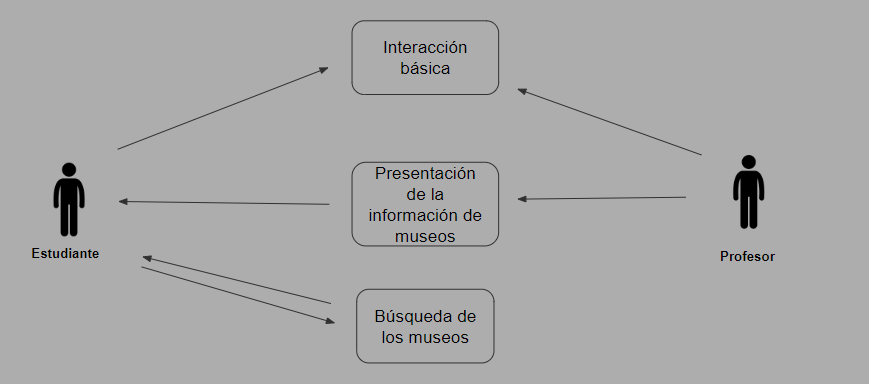
\includegraphics[width=15cm]{imgs/CasoUso_5.PNG}}
\caption{Diagrama Caso 1.5}
\label{fig_5_1}
\end{figure}

\paragraph{Modelo Conceptual}

\begin{figure}[H]
\centerline{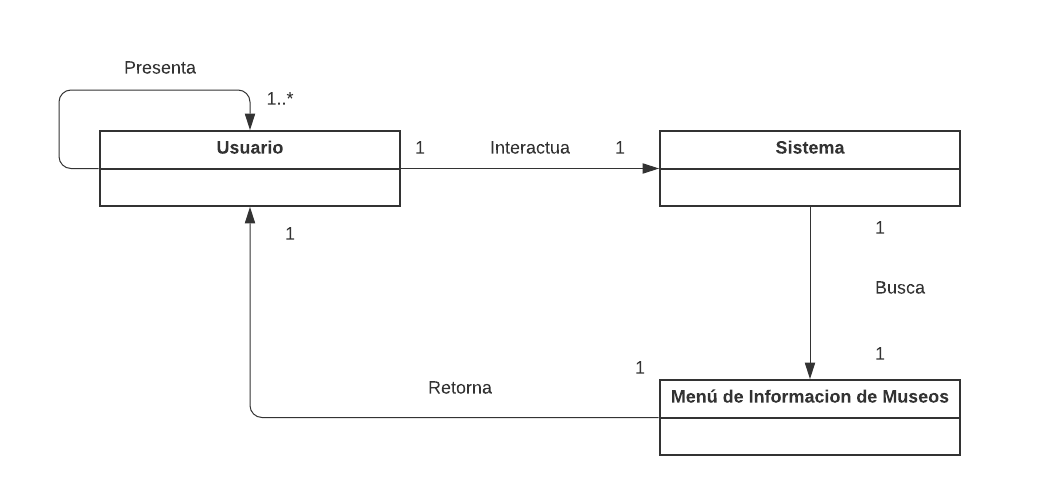
\includegraphics[width=15cm]{imgs/ModeloConceptualCaso_5_3.png}}
\caption{Modelo Conceptual Caso 1.5}
\label{fig_5_2}
\end{figure}

\paragraph{Diagrama de Secuencia o Colaboración}

\begin{figure}[H]
\centerline{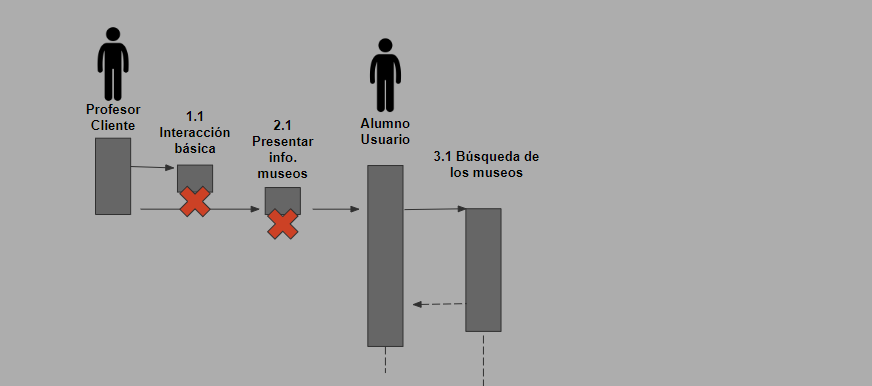
\includegraphics[width=15cm]{imgs/CasoUso_5_2.PNG}}
\caption{Diagrama de Secuencia Caso 1.5}
\label{fig_5_3}
\end{figure}

\paragraph{Priorización}
{\textbf {Tipo:}}
Principal.